This chapter examines existing approaches that are relevant to secure AI-driven DeFi execution. The purpose of this chapter is to understand which parts of the problem are already addressed by existing research and technologies, and where limitations remain. The analysis covers the complete path from interpreting a natural-language request to validating and controlling a blockchain transaction.

First, a set of problem-driven requirements is defined to provide a common basis for evaluation. The chapter then reviews five main approach categories: execution layer security, AI agent blockchain execution, retrieval-based approaches, graph-based approaches, and smart contract security analysis. These approaches are compared against the defined requirements to identify their strengths and limitations. Finally, the chapter discusses the remaining gap between AI generated intent and trusted blockchain execution, which provides the basis for the concept developed in the following chapter.

% ============================================================
% Requirements Analysis
% ============================================================

\section{Requirements Analysis}
\label{sec:requirements_analysis}

The requirements in this section are derived from the problems and objectives
identified in Chapter~\ref{chap:introduction}. They describe the capabilities
that an ideal solution should provide in order to address the problem of
AI-driven DeFi execution.

The main problem is that an AI-generated blockchain action may be technically
executable while still being inconsistent with the user's intended action.
A natural-language request may be incomplete or ambiguous, and the execution
information generated from it may contain an incorrect protocol, contract,
function, asset, pool, reserve, or other protocol-specific relationship. A second concern is that verification itself depends on trustworthy information.
A verification mechanism cannot reliably identify an incorrect execution path
if the information used as its reference is outdated, untrusted, or cannot be
associated with a particular protocol deployment or blockchain network.

Finally, detecting an incorrect action is useful only when the verification
result affects execution. A rejected action must not continue toward blockchain
submission, while an approved action should remain limited to the conditions
that were actually verified.

Based on these problems, six requirements are defined. They cover the complete
path from representing the user's request, through verification, to controlled
execution. The requirements are intentionally independent of the proposed
implementation. Technologies such as Neo4j, Cypher, ERC-4337, a particular
Large Language Model (LLM), or specific protocol APIs are therefore not
requirements themselves. They are implementation choices discussed in later
chapters.

Table~\ref{tab:requirements_overview} summarises the requirements.

\begin{table}[H]
\centering
\small
\begin{tabular}{p{0.8cm} p{3.7cm} p{8.7cm}}
\hline
\textbf{ID} & \textbf{Requirement} & \textbf{Problem Addressed} \\ \hline

R1 &
Complete and unambiguous structured intent &
Natural-language requests may be incomplete, ambiguous, or unsuitable for
direct transaction processing. \\

R2 &
Intent-to-execution relationship validation &
Individually valid protocol, contract, function, and asset information may
still form an incorrect execution path. \\

R3 &
Authoritative and maintainable verification knowledge &
Verification may produce incorrect results when its reference information is
untrusted, outdated, or cannot be associated with the correct network or
protocol deployment. \\

R4 &
Pre-execution enforcement and controlled execution &
Detecting an invalid action does not protect the user if the action can still
be executed, while unrestricted wallet authority introduces an additional
execution risk. \\

R5 &
Traceable verification result &
An approval or rejection is difficult to inspect when the reason for the
verification decision cannot be identified. \\

R6 &
Bounded verification time &
A pre-execution verification mechanism may become unsuitable for interactive
use if it introduces excessive processing delay. \\

\hline
\end{tabular}
\caption{Requirements for secure AI-driven DeFi execution}
\label{tab:requirements_overview}
\end{table}


% ============================================================
% Assessment Method
% ============================================================


\subsection{Assessment Method}
\label{subsec:requirements_assessment_method}

The requirements are used to assess the existing approaches
reviewed in this chapter. For R1 to R5, a four-level star scale
is applied using the requirement-specific criteria defined
in the following subsections. Each requirement contains four
criteria. As summarised in Table~\ref{tab:general_assessment_scale},
four supported criteria result in three stars, three in
two stars, one or two in one star, and none in zero stars.
Mandatory criteria may limit the maximum rating even when
other criteria are satisfied.

\begin{table}[H]
\centering
\small
\begin{tabular}{p{1.5cm} p{3.5cm} p{8.3cm}}
\hline
\textbf{Rating} &
\textbf{Coverage Level} &
\textbf{General Assessment Condition} \\ \hline

$\star\star\star$ & Strong coverage &
All four assessment criteria are supported. \\

$\star\star\circ$ & Substantial coverage &
Three of the four assessment criteria are supported. \\

$\star\circ\circ$ & Limited coverage &
One or two assessment criteria are supported. \\

$\circ\circ\circ$ & No coverage &
None of the assessment criteria are supported. \\

\textit{N/E} & Not evaluable &
Insufficient evidence is available for a reliable assessment. \\

\hline
\end{tabular}
\caption{General assessment scale for qualitative requirements}
\label{tab:general_assessment_scale}
\end{table}

Ratings are based on capabilities demonstrated in the
reviewed literature rather than those requiring additional,
unspecified components. Since each approach group contains
different systems, its assessment reflects documented
characteristic capabilities of the group. Features
demonstrated only by individual representatives are
distinguished from general group capabilities. A criterion
is counted as supported only when the reviewed evidence
justifies its inclusion in the group-level assessment.

R6 is assessed separately using quantitative latency
thresholds. Where the available evidence does not allow
a reliable assessment, the result is marked as
\textit{N/E} rather than treating missing evidence as
demonstrated failure. The State of the Art assessment
relies on published evidence, while the proposed prototype
is assessed through experiments and measurements in the
Evaluation chapter ~\ref{chap:evaluation}. The criterion-level evidence supporting the group ratings
is documented in Appendix~\ref{app:requirement_assessment}.




% ============================================================
% R1
% ============================================================

\subsection{R1: Complete and Unambiguous Structured Intent}
\label{subsec:r1_structured_intent}

\paragraph{Problem.}

Users normally express DeFi actions in natural language. For example:

\begin{quote}
``Supply 100 USDT to Aave V3.''
\end{quote}

Although this request is understandable to a human, it is not yet suitable for
transaction processing. A software system first needs a machine-readable
representation of the requested action. The difficulty is not limited to extracting words or values. The representation
must also contain the information required for the requested action and must
identify when important information is missing or ambiguous.

For example:

\begin{quote}
``Swap WETH for USDT.''
\end{quote}

does not specify the amount to be swapped. Depending on the context, the
blockchain network may also be unclear. Similarly, a token symbol alone does
not necessarily identify a unique blockchain asset. If an AI agent silently guesses such information, the resulting transaction
may differ from what the user intended.

\paragraph{Requirement.}

The system shall transform the user's natural-language request into a complete
and unambiguous machine-readable intent before execution-specific information
is selected.

Depending on the requested action, the structured intent may contain:

\begin{itemize}
    \item the requested action;
    \item the selected protocol;
    \item the blockchain network;
    \item the involved asset or assets;
    \item the amount;
    \item the recipient or spender; and
    \item additional action-specific user parameters.
\end{itemize}

The mandatory information depends on the requested operation. A swap requires
an input and output asset. A transfer requires a recipient. A token approval
requires a spender. A lending operation may require an asset and an operation
such as supply, withdraw, borrow, or repay. R1 does not require the language-processing component to determine the final
smart-contract address, callable function, liquidity pool, reserve, or complete
transaction payload. These execution-specific elements are addressed by R2.

\paragraph{Assessment criteria.}

R1 is assessed using the following criteria:

\begin{enumerate}
    \item[\textbf{C1}] The approach transforms a natural-language request
    into a machine-readable representation.

    \item[\textbf{C2}] The representation identifies the requested action
    and its action-specific mandatory information.

    \item[\textbf{C3}] Missing or invalid mandatory information is detected.

    \item[\textbf{C4}] Ambiguous critical information leads to clarification
    or rejection instead of silent guessing.
\end{enumerate}


% C1 and C2 are mandatory because they represent the minimum functionality required for structured intent generation.

The general scale in Table~\ref{tab:general_assessment_scale} applies.
C1 and C2 are mandatory for a rating above
$\star\circ\circ$, because they represent the minimum functionality required for structured intent generation.


Missing information may be resolved through an explicitly
defined application policy where appropriate. Such defaults
must be applied consistently and distinguished from values
inferred without sufficient information. Ambiguities that
cannot be resolved through a defined policy require
clarification or rejection.

% ============================================================
% R2
% ============================================================

\subsection{R2: Intent-to-Execution Relationship Validation}
\label{subsec:r2_execution_relationship}

\paragraph{Problem.}

A complete structured intent does not guarantee that the execution information
selected for it is correct. Different pieces of information may be individually
valid while still forming an incorrect combination.

For example, an AI agent may correctly identify Aave V3, USDT, and a supply
operation but still select a contract or function that does not belong to the
intended Aave V3 supply operation. Such a transaction may still be technically executable. Technical validity
alone therefore does not prove that the selected execution information
correctly represents the user's intent.

In Web3, DeFi operations are performed through identifiable on-chain entities.
A wallet interacts with a contract at a particular address, calls a particular
function, and supplies parameters such as token addresses and amounts.
Protocols such as Uniswap and Aave expose their operations through
protocol-specific contracts, pools, markets, and supported assets
\cite{uniswapDocs,aaveV3OverviewDocs}.

For this thesis, a \textit{relationship} describes an explicit association
between entities that are expected to belong together for a particular
execution.

Examples include:

\begin{itemize}
    \item a protocol deployment supporting a particular action;
    \item an action being executed through an official contract;
    \item a contract exposing the required function;
    \item a lending market supporting a particular reserve asset; and
    \item a liquidity pool supporting the required token pair.
\end{itemize}

\paragraph{Requirement.}

The system shall validate that the execution information selected for the
structured intent forms the expected action-specific relationship before
blockchain execution.

A simplified execution relationship can be represented as:


\begin{figure}[H]
\centering
\resizebox{\linewidth}{!}{%
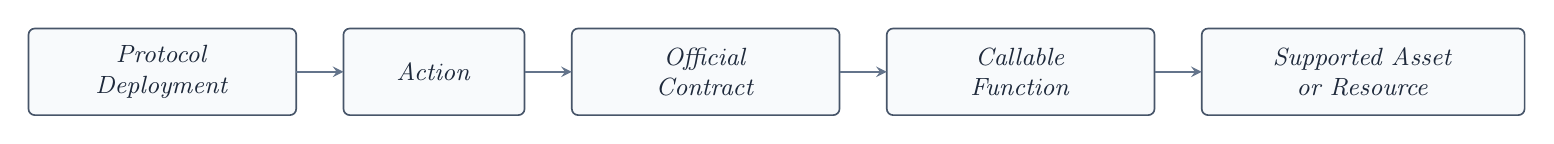
\begin{tikzpicture}[x=1cm,y=1cm,>=stealth]

% Colours
\definecolor{stepfill}{HTML}{F8FAFC}
\definecolor{stepborder}{HTML}{475569}
\definecolor{arrowcol}{HTML}{64748B}
\definecolor{steptext}{HTML}{1E293B}

% Protocol Deployment
\draw[rounded corners=0.08cm, draw=stepborder,
      fill=stepfill, line width=0.6pt]
  (0,0) rectangle (3.4,1.1);
\node[align=center, text=steptext, font=\small]
  at (1.7,0.55)
  {\textit{Protocol}\\\textit{Deployment}};

% Action
\draw[rounded corners=0.08cm, draw=stepborder,
      fill=stepfill, line width=0.6pt]
  (4.0,0) rectangle (6.3,1.1);
\node[align=center, text=steptext, font=\small]
  at (5.15,0.55)
  {\textit{Action}};

% Official Contract
\draw[rounded corners=0.08cm, draw=stepborder,
      fill=stepfill, line width=0.6pt]
  (6.9,0) rectangle (10.3,1.1);
\node[align=center, text=steptext, font=\small]
  at (8.6,0.55)
  {\textit{Official}\\\textit{Contract}};

% Callable Function
\draw[rounded corners=0.08cm, draw=stepborder,
      fill=stepfill, line width=0.6pt]
  (10.9,0) rectangle (14.3,1.1);
\node[align=center, text=steptext, font=\small]
  at (12.6,0.55)
  {\textit{Callable}\\\textit{Function}};

% Supported Asset or Resource
\draw[rounded corners=0.08cm, draw=stepborder,
      fill=stepfill, line width=0.6pt]
  (14.9,0) rectangle (19.0,1.1);
\node[align=center, text=steptext, font=\small]
  at (16.95,0.55)
  {\textit{Supported Asset}\\\textit{or Resource}};

% Arrows
\draw[->, line width=0.7pt, draw=arrowcol]
  (3.4,0.55) -- (4.0,0.55);

\draw[->, line width=0.7pt, draw=arrowcol]
  (6.3,0.55) -- (6.9,0.55);

\draw[->, line width=0.7pt, draw=arrowcol]
  (10.3,0.55) -- (10.9,0.55);

\draw[->, line width=0.7pt, draw=arrowcol]
  (14.3,0.55) -- (14.9,0.55);

\end{tikzpicture}%
}
\caption{Simplified action-oriented relationship path used for verification.}
\label{fig:action_oriented_relationship}
\end{figure}


The exact relationship depends on the requested action. A swap may additionally
require verification of a router, token pair, and corresponding liquidity pool.
A lending action may require verification of the protocol deployment, Pool
contract, lending function, and reserve asset. R2 does not prescribe a particular verification technology. Relationships may
be checked using structured rules, registries, policy engines, graph structures,
or another suitable mechanism.

\paragraph{Assessment criteria.}

R2 is assessed using the following criteria:

\begin{enumerate}
    \item[\textbf{C1}] The selected protocol deployment is checked against
    the requested action.

    \item[\textbf{C2}] The target contract and callable function are checked
    against the requested action.

    \item[\textbf{C3}] The required asset, pool, reserve, market, or other
    protocol-specific resource is checked against the selected action and
    deployment.

    \item[\textbf{C4}] The relationship validation is performed before
    blockchain execution.
\end{enumerate}



The general scale in Table~\ref{tab:general_assessment_scale} applies.
C4 is mandatory for a rating above $\star\circ\circ$ because R2 concerns
pre-execution validation rather than analysis of an already executed transaction.

% ============================================================
% R3
% ============================================================

\subsection{R3: Authoritative and Maintainable Verification Knowledge}
\label{subsec:r3_verification_knowledge}

\paragraph{Problem.}

The correctness of a verification decision depends on the information used as
the reference for that decision.

For example, checking whether a contract belongs to Aave V3 is useful only when
the expected contract information itself is trustworthy. An outdated contract
address, incorrect token mapping, wrong protocol version, or stale pool or
reserve relationship may lead to an incorrect verification result even when the
verification logic itself operates correctly. This problem is particularly relevant in DeFi because execution information may
differ between blockchain networks and protocol versions. Supported assets,
pools, reserves, and protocol deployments may also change over time. Verification knowledge must therefore have an identifiable origin and must be
maintainable when the supported environment changes.

\paragraph{Requirement.}

The system shall obtain verification information from identifiable trusted or
authoritative sources and shall retain sufficient context to determine where
the information originated and to which deployment it applies.

The system shall also allow outdated or changed verification information to be
updated or invalidated without redesigning the complete verification mechanism.

Relevant context may include:

\begin{itemize}
    \item the information source;
    \item blockchain network;
    \item protocol and protocol version;
    \item contract or asset address;
    \item synchronization or retrieval time; and
    \item validity or active status.
\end{itemize}

R3 does not require the use of a particular API or data-storage technology.
For example, a solution may obtain information from official protocol APIs,
deployment registries, verified on-chain data, protocol documentation, or
another identifiable authoritative source. R3 does not prescribe a particular information source,
synchronisation method, or data-storage technology.
The mechanisms selected to address this requirement
are discussed in the Concept and Implementation chapters.


\paragraph{Assessment criteria.}

R3 is assessed using the following criteria:

\begin{enumerate}
    \item[\textbf{C1}] Verification information originates from defined
    trusted or authoritative sources.

    \item[\textbf{C2}] The origin and relevant context of the verification
    information can be identified, including information such as source,
    network, or protocol version where applicable.

    \item[\textbf{C3}] Changed, outdated, or removed verification information
    can be updated or invalidated.

    \item[\textbf{C4}] Additional supported entities or relationships can be
    incorporated without redesigning the complete verification mechanism.
\end{enumerate}


The general scale in Table~\ref{tab:general_assessment_scale} applies.
C1 is mandatory for a rating above $\star\circ\circ$ because verification
knowledge must originate from an identifiable trusted or authoritative source.

For assessment, the accepted sources and the basis for treating them as
trusted or authoritative shall be stated explicitly. Source authority
shall be assessed for the relevant information and deployment context;
retrieval relevance or the presence of information in a knowledge base
alone does not establish authority.
% ============================================================
% R4
% ============================================================

\subsection{R4: Pre-Execution Enforcement and Controlled Execution}
\label{subsec:r4_enforcement}

\paragraph{Problem.}

Identifying an incorrect or unverifiable action does not protect the user if the
action can still proceed to signing or blockchain submission.

For example, a verification mechanism may correctly detect that the selected
contract does not belong to the requested protocol. If this result is presented
only as a warning while the transaction remains executable, the verification
mechanism does not provide an effective security boundary. A second problem occurs after an action has been approved. Approval of one
verified action should not provide an automated agent with unrestricted
authority over the user's wallet. The execution should remain limited to the
conditions that were verified.

\paragraph{Requirement.}

The system shall prevent rejected or unresolved actions from continuing toward
blockchain execution and shall allow approved actions to execute only under
defined execution restrictions.

The expected process is:

\begin{enumerate}
    \item the required verification checks are completed;
    \item an explicit approval or rejection is produced;
    \item rejected or unresolved actions are prevented from continuing;
    \item only approved actions are passed to the execution mechanism; and
    \item approved actions remain restricted to the verified execution
    conditions.
\end{enumerate}

Relevant restrictions may include permitted target contracts,
    permitted callable functions,
     transaction or spending limits,
    permitted recipients or spenders,
     blockchain-network restrictions,
    time-limited permissions and
    revocable delegated permissions. Programmable smart-account architectures can support such execution controls.
ERC-4337, for example, separates UserOperation validation from execution and
allows smart-account implementations to define their own validation logic
\cite{buterinERC4337AccountAbstraction2021,
linMeasurementInvestigationERC43372024}.

R4 does not require ERC-4337 specifically. The requirement concerns the
enforcement of the verification decision and controlled execution of an
approved action.

\paragraph{Assessment criteria.}

R4 is assessed using the following criteria:

\begin{enumerate}
    
\item[\textbf{C1}] An explicit verification outcome
is produced before blockchain execution, distinguishing
approval, rejection, and insufficient evidence.

\item[\textbf{C2}] Rejected or unresolved actions are
automatically prevented from continuing toward execution.


    \item[\textbf{C3}] Approved actions execute only within restrictions
that enforce the applicable verified execution conditions.

\item[\textbf{C4}] The executed operation remains bound to the approved
security-relevant parameters. Changes to these parameters require
revalidation of the modified operation before execution.
\end{enumerate}


The general scale in Table~\ref{tab:general_assessment_scale} applies.
C2 and C3 are mandatory for a rating above $\star\circ\circ$ because
the requirement covers enforcement of
negative decisions and controlling approved
execution.

% ============================================================
% R5
% ============================================================

\subsection{R5: Traceable Verification Result}
\label{subsec:r5_traceability}

\paragraph{Problem.}

A verification decision is difficult to inspect when the system returns only an
unexplained approval or rejection.

For example:

\begin{quote}
``Transaction rejected.''
\end{quote}

does not indicate whether the rejection was caused by the protocol, contract,
function, asset, amount, recipient, or another verification condition. This is particularly important when an AI-generated action appears reasonable
to the user but is rejected by the verification mechanism. The user, developer,
or evaluator should be able to identify which verification condition produced
the decision.

\paragraph{Requirement.}

The system shall provide a structured and traceable
verification result that identifies the outcome and
the conditions responsible for it. This includes
approval, rejection, and cases where sufficient
verification evidence is unavailable. The underlying result shall contain sufficient
information to identify the relevant verification
condition, entity, or relationship. Where applicable,
the expected and observed values shall be available
to support inspection of the decision.

For example, instead of returning only:

\begin{quote}
``Transaction rejected.''
\end{quote}

the system may report:

\begin{quote}
``Contract mismatch: the selected address does not match the expected contract
for the selected protocol deployment.''
\end{quote}

\paragraph{Assessment criteria.}

R5 is assessed using the following criteria:

\begin{enumerate}
    
\item[\textbf{C1}] The verification outcome,
including approval, rejection, or insufficient evidence,
is explicitly reported.

    \item[\textbf{C2}] A reason or stable verification identifier is
    provided.

    \item[\textbf{C3}] The specific field, rule, entity, or relationship
    responsible for the result can be identified.

    \item[\textbf{C4}] When a mismatch occurs, the expected and observed
    values are available when both values can be determined.
\end{enumerate}


The general scale in Table~\ref{tab:general_assessment_scale} applies.
C3 is mandatory for a rating above $\star\circ\circ$ because a traceable
result must identify the verification condition responsible for the decision.
% ============================================================
% R6
% ============================================================

\subsection{R6: Bounded Verification Time}
\label{subsec:r6_latency}

\paragraph{Problem.}

The verification mechanism is positioned before blockchain execution and
therefore introduces an additional processing step into every protected
transaction.

Even if the verification decision is correct, an excessively slow verification
process may make the system unsuitable for interactive use. Terms such as
``fast'' or ``low latency'' are therefore insufficient unless the expected
processing time can be measured.

\paragraph{Requirement.}

Pre-execution verification introduces additional processing
time into an interactive transaction workflow. To assess
this overhead, the thesis defines the following
prototype-specific acceptance target:

\begin{quote}
At least 95\% of pre-execution verification decisions
shall be returned within 2 seconds.
\end{quote}

The measurement begins when a complete structured intent
reaches the verification stage and ends when the structured
verification result becomes available. It excludes
natural-language processing, user interaction, wallet
confirmation, bundler processing, and blockchain submission
and confirmation times. The threshold is an evaluation target selected for this
prototype rather than a universal performance requirement.
Existing approaches are rated only when their reported
measurements are comparable with this measurement boundary.
Otherwise, the result is marked as \textit{N/E}.

\begin{table}[H]
\centering
\begin{tabular}{p{2.3cm} p{9.9cm}}
\hline
\textbf{Rating} & \textbf{Assessment Condition} \\ \hline

$\star\star\star$ &
At least 95\% of comparable pre-execution verification decisions complete
within 2 seconds. \\

$\star\star\circ$ &
At least 90\% but fewer than 95\% of comparable verification decisions complete
within 2 seconds. \\

$\star\circ\circ$ &
At least 75\% but fewer than 90\% of comparable verification decisions complete
within 2 seconds. \\

$\circ\circ\circ$ &
Fewer than 75\% of comparable verification decisions complete within
2 seconds, or the approach is explicitly designed only for offline or
post-execution analysis. \\


\hline
\end{tabular}
\caption{Assessment scale for R6: Bounded verification time}
\label{tab:r6_scale}
\end{table}


The following section reviews existing approaches and evaluates them against
these six requirements.